\documentclass[
	ngerman,%globale Übergabe der Hauptsprache
%	logofile=example-image, %Falls die Logo Dateien nicht vorliegen
	authorontitle=true,
	]{bfhbeamer}


%\usepackage[main=ngerman]{babel}

% Der folgende Block ist nur bei pdfTeX auf Versionen vor April 2018 notwendig
\usepackage{iftex}
\ifPDFTeX
\usepackage[utf8]{inputenc}%kompatibilität mit TeX Versionen vor April 2018
\fi
\usepackage{bytefield}
\usepackage{pifont}
\usepackage{xcolor}
\usepackage{fontawesome5}
\usepackage{todonotes}
\usepackage{hyperref}
\usepackage{graphicx}
\usepackage{subfigure}
\usepackage{tikz}
\usetikzlibrary{positioning}

%Makros für Formatierungen der Doku
%Im Allgemeinen nicht notwendig!
\let\code\texttt

\title{Swiss Army Knife Network Sniffer (NSAK) }
\subtitle{Version 0.4}
\author[]{Lukas von Allmen (vonal3) and Frank Gauss (gausf1)}
\institute{Bern University of Applied Sciences}
\titlegraphic*{\includegraphics{{assets/swiss-army-network-sniffer}}}%is only used with BFH-graphic and BFH-fullgraphic

%Activate the output of a frame number:
\setbeamertemplate{section page}[BFH-ruled]
\setbeamertemplate{page number in head/foot}[framenumber]
\AtBeginSection{\sectionpage}

\begin{document}

%\maketitle

%second title variant
%\setbeamertemplate{title page}[BFH-Orange]

%\maketitle

\setbeamertemplate{title page}[BFH-graphic]
\maketitle

%\setbeamertemplate{title page}[BFH-fullgraphic]
%\maketitle

\section{Introduction}\label{sec:introduction}

\begin{frame}{Motivation}
	\framesubtitle{Subtitle}
	\begin{itemize}
		\item \textbf{Cyberangriffe nehmen zu}
		\small Angriffsbarrieren sinken, Automatisierung steigt
		\vspace{0.3em}

		\item \textbf{Sicherheit erfordert Sichtbarkeit}
		\small Netzwerkangriffe sind oft nur auf Layer 2–4 erkennbar
		\vspace{0.3em}

		\item \textbf{Bestehende Frameworks sind komplex}
		\small Hoher Konfigurations- und Betriebsaufwand
		\vspace{0.3em}

		\item \textbf{Unser Ansatz (PoC)}
		\small Modularer, kontrollierter Network-Sniffer für Angriffsszenarien


	\end{itemize}
	Eher alles als Bilder
	(Franky)
\end{frame}


\section{Design and Architecture}\label{sec:design-and-architecture}
\newcommand\frametab{\tabto{2.25cm}}

\begin{frame}{NSAK Design and Architecture Overview}
    \framesubtitle{Resources}

    \vspace{0.4em}
    \begin{itemize}
        \item[\faServer]{
            \textbf{Devices}\\
            \vspace{0.4em}
            Physical or virtual machines, which can be provisioned as a NSAK device
            \vspace{0.6em}
        }
        \item[\faNetworkWired]{
            \textbf{Environments}\\
            \vspace{0.4em}
            Network topology incl. infrastructure components, servers, clients and services
            \vspace{0.6em}
        }
        \item[\faLayerGroup]{
            \textbf{Scenarios}\\
            \vspace{0.4em}
            Designed to be run in environements, consisting of a sequence of drills
            \vspace{0.6em}
        }
        \item[\faCogs]{
            \textbf{Drills}\\
            \vspace{0.4em}
            Reusable building blocks for configuration, reconnaissance or exploitation
            \vspace{0.6em}
        }
    \end{itemize}
    \vspace{0.8em}
\end{frame}


\section{Hardware Evaluation}\label{sec:hardware-evaluation}
\begin{frame}{Hardware Selection}


\begin{columns}[T,onlytextwidth]

	% -------- Banana Pi --------
	\column{0.5\textwidth}

	\textbf{Banana Pi R4 Pro}

	\vspace{0.5em}
	\includegraphics[width=0.6\linewidth]{assets/banana-pi}

	\vspace{0.5em}
	\scriptsize
	\begin{itemize}
		\item RAM: 8 GB
		\item CPU: Quad-Core ARM
		\item Ports: 4\times 1~\amp~2\times 10 GbE
		\item Wi-Fi: Optional with a module
	\end{itemize}

	% -------- NanoPi --------
	\column{0.5\textwidth}

	\textbf{NanoPi R76S}

	\vspace{0.5em}
	\includegraphics[width=0.45\linewidth]{assets/nano-pi}

	\vspace{0.5em}
	\scriptsize
	\begin{itemize}
		\item RAM: 16 GB
		\item CPU: Octa-Core ARM
		\item Ports: 2\times 2.5 GbE
		\item Wi-Fi: Optional with a module
	\end{itemize}

\end{columns}

\end{frame}


\section{Implementation}\label{sec:implementation}
\begin{frame}{NSAK Framework Implementation}
    \framesubtitle{Components, stack, dependencies}

    \begin{columns}[T]
        \begin{column}{0.52\textwidth}
            \textbf{Framework (Monorepo)}
            \begin{itemize}
                \item \textbf{Core}: framework logic
                \item \textbf{CLI}: user interaction
                \item \textbf{Resource Library}: devices, environments, scenarios, drills
            \end{itemize}

            \vspace{0.4em}
            \textbf{System Dependencies}
            \begin{itemize}
                \item Python Toolchain: \texttt{python3}, \texttt{uv}
                \item OCI Containers: \texttt{podman}, \texttt{podman-compose}
                \item Net Control: \texttt{iptables}/\texttt{nftables}
            \end{itemize}
        \end{column}

        \begin{column}{0.48\textwidth}
            \textbf{Python Dependencies}
            \begin{itemize}
                \item \textbf{Quality}: \texttt{ruff}, \texttt{mypy}, \texttt{pre-commit}
                \item \textbf{Testing}: \texttt{pytest}
                \item \textbf{Pre-commit}: \textbf{rule enforcement}
                \item \textbf{Config}: \texttt{pyyaml}
                \item \textbf{Networking}: \texttt{scapy}
                \item \textbf{CLI}: \texttt{click}
            \end{itemize}
        \end{column}
    \end{columns}
\end{frame}

\begin{frame}{MITM Scenario Implementation}
    \framesubtitle{ARP spoofing \& transparent TCP proxy}

    \begin{columns}[T]
        \begin{column}{0.52\textwidth}
            \textbf{Drills}
            \begin{enumerate}
                \item \textbf{Discover hosts} \textit{\scriptsize scan target network}
                \item \textbf{ARP spoof} \textit{\scriptsize discover hosts, poison ARP tables}
                \item \textbf{Transparent TCP proxy}
                \begin{itemize}
                    \item \scriptsize Client+server sockets for interception
                    \item \scriptsize Redirect traffic via \texttt{iptables}/\texttt{nftables}
                    \item \scriptsize Read~\&~modify forwarded packets
                \end{itemize}
            \end{enumerate}

            \vspace{0.6em}
            \textbf{Environment}
            \begin{itemize}
                \item \textbf{Simulation:} \texttt{podman-compose}
                \item \textbf{Physical lab:} 2\times Raspberry Pi~\&~switch
            \end{itemize}
        \end{column}

        \begin{column}{0.48\textwidth}
            \centering
            \includegraphics[width=\linewidth]{assets/mitm_arp_spoofing_transparent_tcp_proxy}

            \vspace{0.4em}
            {\scriptsize\textit{Simple TCP Client–Server Lab}}

            \vspace{0.6em}
            \href{assets/nsak_mitm_scenario.mp4}{\beamergotobutton{Demo video}}
        \end{column}
    \end{columns}
\end{frame}

\begin{frame}{Rogue AP – Drill Order}
	\framesubtitle{Controlled Wi-Fi Scenario}

	\begin{columns}[T,onlytextwidth]



		% -------- Rechte Spalte: Bild --------
		\column{0.60\textwidth}
		\centering
		\includegraphics[width=0.7\linewidth]{assets/rogue-ap}
			% -------- Linke Spalte: Drill Timeline --------
		\column{0.9\textwidth}

		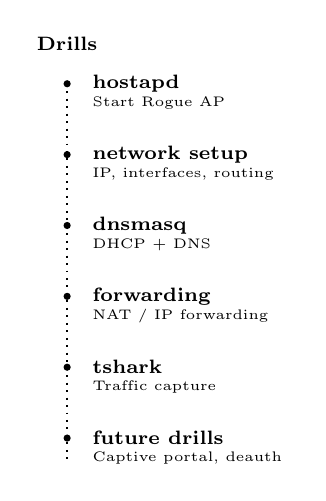
\begin{tikzpicture}[transform shape]
			\node[anchor=south] at (0,0.3) {\scriptsize\textbf{Drills}};

			% Linie
			\draw[dotted, line width=0.7pt] (0,0) -- (0,-4.8);

			% Punkte + Labels
			\foreach \y/\title/\desc in {
				0/{hostapd}/{Start Rogue AP},
				-0.9/{network setup}/{IP, interfaces, routing},
				-1.8/{dnsmasq}/{DHCP + DNS},
				-2.7/{forwarding}/{NAT / IP forwarding},
				-3.6/{tshark}/{Traffic capture},
				-4.5/{future drills}/{Captive portal, deauth}
			}{
				\fill (0,\y) circle (1.3pt);
				\node[anchor=west] at (0.20,\y) {\scriptsize\textbf{\title}};
				\node[anchor=west, align=left] at (0.20,\y-0.25) {\tiny \desc};
			}
		\end{tikzpicture}

	\end{columns}
\end{frame}


\section{Evaluation and Discussion}\label{sec:evaluation_and_discussion}

\begin{frame}{Future Work and Conclusion}
	\framesubtitle{Key Insights and Takeaways}

	\begin{columns}[T]
		\begin{column}{0.5\textwidth}
			Future Work
			\vspace{0.4em}
			\begin{itemize}
				\item[\faCloud] REST API: Integration of frontends or systems
				\vspace{0.4em}
				\item[\faReact] GUI: Better UX and lower entry barrier
				\vspace{0.4em}
				\item[\faBroom] Redesign cleanup management
				\vspace{0.4em}
				\item[\faCogs] Implement configuration management
				\vspace{0.4em}
				\item[\faBug] Test coverage: Correctness and maintainability
				\vspace{0.4em}
				\item[\faShieldVirus] Security Concept: NSAK must be secure
				\vspace{0.4em}
			\end{itemize}
		\end{column}
		\begin{column}{0.5\textwidth}
			Conclusion\\
			\vspace{0.4em}
			\small We could show the feasibility of a PoC realization of a Network Swiss Army Knife (NSAK) and that the modular drills can be combined to effectively build scenarios, which can be executed on constraint hardware in simulated or real-world network environments.\\
			\vspace{0.4em}
			\small The key difficulty is that the automation of scenarios requires a lot of assumptions about the target environment, which potentially renders them very brittle.


%			\begin{itemize}
%				\item Design and implementation of the framework
%				\item Evaluated and configured devices
%				\item Implemented environments, scenarios, drills
%				\item Putting everything together
%				\item Run scenarios in physical and simulated environments
%			\end{itemize}
		\end{column}
	\end{columns}
	\centering
\end{frame}


\section[Access Point Demo: Can you spot the rougue AP? / Open questions?]{Access Point Demo: Can you spot the rogue AP?\\~\\ Open questions?}\label{sec:demo-access-point-and-questions}


\end{document}
